%%%%%%%%%%%%%%%%%%%%%%%%%%%%%%%%%%%%%%%%%
%
% CMPT 435
% Spring 2019
% Lab One
%
%%%%%%%%%%%%%%%%%%%%%%%%%%%%%%%%%%%%%%%%%

%%%%%%%%%%%%%%%%%%%%%%%%%%%%%%%%%%%%%%%%%
% Short Sectioned Assignment
% LaTeX Template
% Version 1.0 (5/5/12)
%
% This template has been downloaded from: http://www.LaTeXTemplates.com
% Original author: % Frits Wenneker (http://www.howtotex.com)
% License: CC BY-NC-SA 3.0 (http://creativecommons.org/licenses/by-nc-sa/3.0/)
% Modified by Alan G. Labouseur  - alan@labouseur.com
%
%%%%%%%%%%%%%%%%%%%%%%%%%%%%%%%%%%%%%%%%%

%----------------------------------------------------------------------------------------
%	PACKAGES AND OTHER DOCUMENT CONFIGURATIONS
%----------------------------------------------------------------------------------------

\documentclass[letterpaper, 10pt]{article} 


\usepackage[english]{babel} % English language/hyphenation
\usepackage[utf8]{inputenc}
\usepackage{graphicx}
\usepackage[lined,linesnumbered,commentsnumbered]{algorithm2e}
\usepackage{listings}
\usepackage{minted}
\usepackage{fancyhdr} % Custom headers and footers
\pagestyle{fancyplain} % Makes all pages in the document conform to the custom headers and footers
\usepackage[table]{xcolor}
\usepackage{csquotes}
\usepackage{natbib}
\usepackage[nottoc]{tocbibind}
\usepackage{lastpage}
\usepackage{url}
\usepackage{float}
\usepackage{scrextend}
\usepackage{epigraph}
\usepackage{tcolorbox}
\usepackage{tabularx}
\fancyhead{} % No page header - if you want one, create it in the same way as the footers below
\fancyfoot[L]{} % Empty left footer
\fancyfoot[C]{page \thepage\ of \pageref{LastPage}} % Page numbering for center footer
\fancyfoot[R]{}
\usepackage{listings}% http://ctan.org/pkg/listings
\usepackage{hyperref}
\renewcommand{\headrulewidth}{0pt} % Remove header underlines
\renewcommand{\footrulewidth}{0pt} % Remove footer underlines
\setlength{\headheight}{13.6pt} % Customize the height of the header
\usepackage{pgfplots}

\pgfplotsset{width=7cm,compat=1.8}

%----------------------------------------------------------------------------------------
%	TITLE SECTION
%----------------------------------------------------------------------------------------

\newcommand{\horrule}[1]{\rule{\linewidth}{#1}} % Create horizontal rule command with 1 argument of height

\title{	
   \normalfont \normalsize 
   \textsc{CMPT 435 - Fall 2020 - Dr. Labouseur} \\[10pt] % Header stuff.
   \horrule{0.5pt} \\[0.25cm] 	% Top horizontal rule
   \large{Semester Project} \\
   \textsc{Pooled Infection Testing Simulator}\\[20pt]% Assignment title
 \author{Sam Alcosser \\ \normalsize Samuel.Alcosser1@Marist.edu}
   \horrule{0.5pt} \\ 	% Bottom horizontal rule
   


	% Today's date.
  
\date{\normalsize\today} 
}
\begin{document}




\fontfamily{bch}\selectfont
\maketitle
\tableofcontents
\newpage




\section{Introduction}

\subsection{History and Background}

With current events in late 2020, we are currently past the point where a test for the novel disease is hard to come by. Although despite this, there is something to be said for the efficiency of the tests. As described by Dr. Alan Labouseur, during the time of WWII, there was a need for a more efficent way to test for infections. One idea was pooled testing. With this approach, instead of handing out individual tests, a set of people would all be swabbed or sampled, all of the samples would be compiled into one testable container, and the container would be tested as a whole. If the test comes back negative, everyone is assumed to be clear, and if not, the sample set is split into two sub samples and repeat the process. After a certain point, the testing facility will decide to go to individual tests to ensure who is actually positve. With this approach, instead of using 1000 tests on 1000 people, the number of tests can sometimes be reduced down to under 250 for the same sample size. Dr. Labouseur's pseudo-code algorithm for this process can be seen below.

\begin{center}
 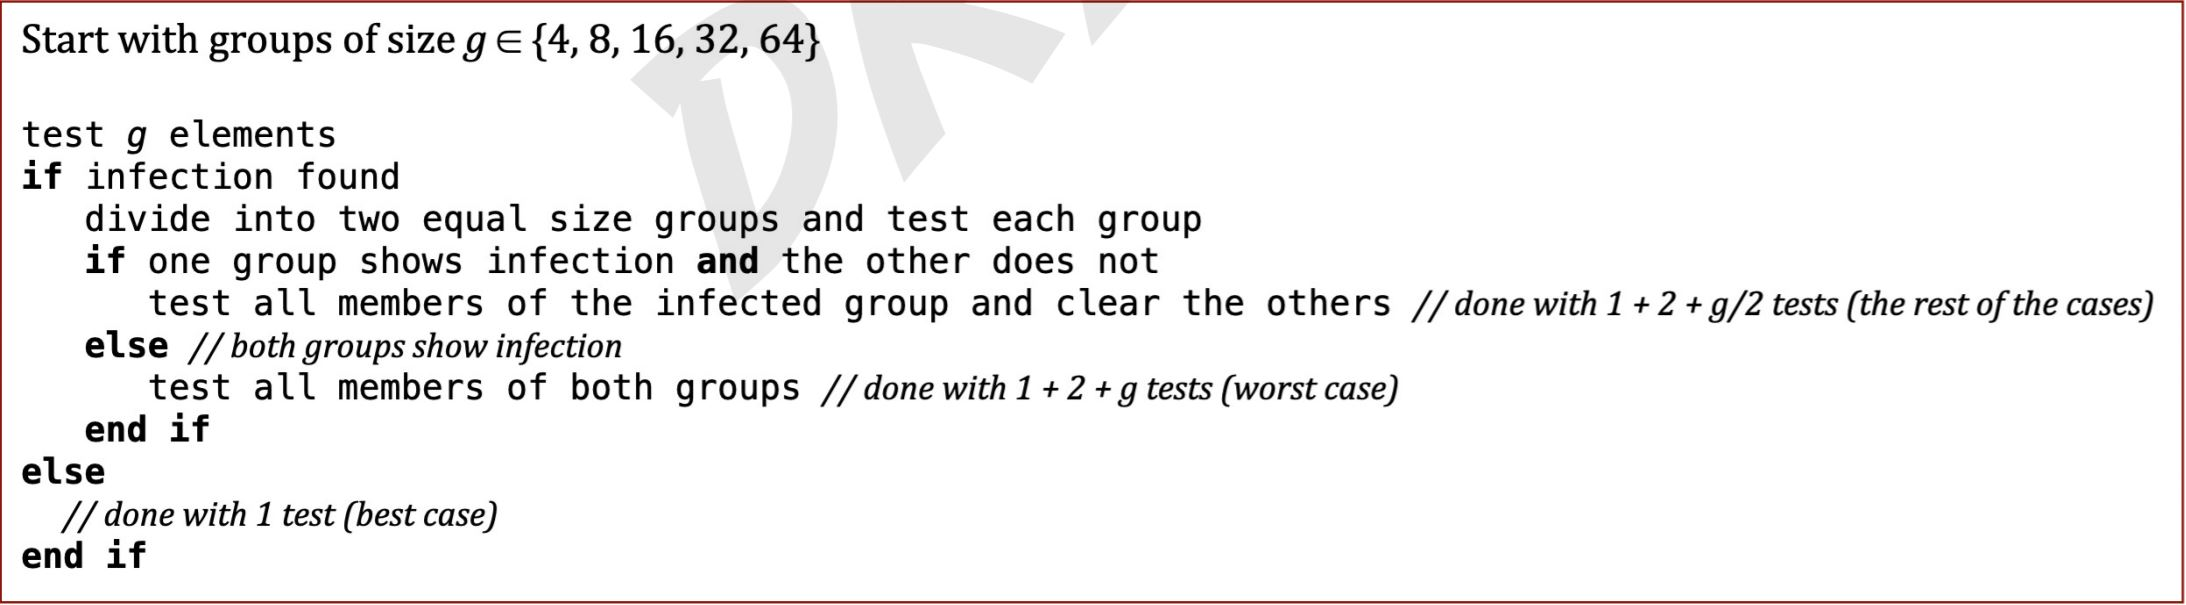
\includegraphics[width=\textwidth ]{pooled testing.JPG}
 \end{center}
 
\subsection{Implementation and Logic Design}

To simulate this situation, I needed three main parts.

\begin{itemize}
    \item A way to set up the sample size with a simulated infection rate, and put them into pools of 8
    \item A way to implement the pooled testing algorithm on each pool
    \item Some way to abstract the use of both of the other parts
\end{itemize}

Also, A very simple UI was created to assist the user in running the simulations. To see how this works, look to the Appendix subsection titled "\texttt{main.cpp} : Making The Simulator Usable".

\section{Implementation}

\subsection{\texttt{PooledTesting::setupPools()} : Setup}

This first function gets called at the beginning of the process. The function takes a population size and a percentage of infection, randomly infects the correct number of people, and loads up the \texttt{testPools} vector with sets of eight people.


 \begin{addmargin}[-5em]{1em}
\begin{small}
\begin{minted}[linenos=true]{cpp}
void PooledTesting::setupPools(double size, double pcPos)
{

    tPeople = size;
    std::vector<int> population(tPeople, 0);
    int numPos = (int)(static_cast<double>(tPeople) * pcPos);

    std::vector<int> indexes;
    int chosen = 0;
    while (chosen < numPos)
    {

        std::random_device dev; 
        std::mt19937 rng(dev());
        std::uniform_int_distribution<std::mt19937::result_type> dist6(0, (tPeople - 1));
        int attempt = dist6(rng);
        if (std::find(indexes.begin(), indexes.end(), attempt) != indexes.end())
        {
            continue;
        }
        else
        {

            indexes.push_back(attempt);
            population[attempt] = 1;
            chosen++;
        }
    }

    int remainder = tPeople % poolSize;

    int pools = (tPeople - remainder) / poolSize;

    for (int i = 0; i < pools; i++)
    {
        std::vector<int> pool;
        for (int j = 0; j < poolSize; j++)
        {
            int subInd = (i * poolSize) + j;
            pool.push_back(population[subInd]);
        }
        testPools.push_back(pool);
    }
    if (remainder > 0)
    {
        int processedCounter = pools * poolSize;
        std::vector<int> remVect;
        for (int x = processedCounter - 1; x < tPeople; x++)
        {
            remVect.push_back(population[x]);
        }
        testPools.push_back(remVect);
    }
    std::cout << testPools.size() << " pools have been set up." << std::endl;
}
\end{minted}
\end{small}
\end{addmargin}

\begin{enumerate}
    \item (lines 4-9): Setup the local variables for this method including:
        \begin{enumerate}
            \item \texttt{tPeople} for the size of the population
            \item \texttt{population} for set of all people in the population in a vector of ints initialized with the population size \texttt{tPeople} each as 0, to indicate starting as negative
            \item \texttt{numPos} for the computed amount of positive cases based on population and the infection rate \texttt{pcPos} which was passed in
            \item \texttt{indexes} for the indexes of the population set which are randomly decided to be positive (also useful to ensure that there are no repeats)
            \item \texttt{chosen} to keep track of how many indexes have been chosen
        \end{enumerate}
    \item While the number of chosen indexes is less than the number of needed positive cases (line 10), create random numbers in the range of the number of people (lines 13-16) and if the number has not been previously chosen, (line 17), add it to the list of selected indexes and mark that index as chosen. Each of the "people" at these indexes will be marked positive by a "1" for their value instead of a "0". (lines 24-26)
    \item Decide the number of needed pools by first stripping off the people that would create an uneven split (line 30),  and then divide the rest of the people by the pool size (line 32).
    \item Create a vector and populate it with 8 "people" of the whole population size an amount of times equivilent to the number of necessary pools. 
        \begin{enumerate}
            \item Start by making an iterator that will run from 0 to right under the number of desired pools (line 34).
            \item Make a vector of ints to hold the current working pool, and fill it with the next eight "people's" values using another iterator from 0 to 7 (line 37). To find the correct index, multiply the index of the pool \texttt{i},  and multiply it by \texttt{poolSize} to account for the previous pools values. Then, add the value of the iterator for the person in the current pool \texttt{j}, and use that value to take the correct index, and push it onto the current pool (lines 39,40).
            \item Once the pool is created, push it onto the vector of pools \texttt{testPools} (line 42).
        \end{enumerate}
    \item Don't forget about the remaining people that couldn't fit into a complete pool. Take them and put them into one final test pool.
        \begin{enumerate}
            \item Start a counter for the correct index by computing the previously processed indexes by setting \texttt{processedCounter} to   \texttt{pools * poolSize}(line 46)
            \item Fill the final pool vector \texttt{remVect} by starting at the index right below the number of processed people, working until the last index (lines 47-51)
            \item Push the final pool vector to \texttt{testPools} and indicate to the user that the pools have been set up. (lines 52,54)
        \end{enumerate}
     
\end{enumerate}

\subsection{\texttt{PooledTesting::itTest} : Testing the Pools}

Now that we have our pools set up, it is time to test the pools for positive cases. Following the algorithm, If a case comes back as positve, it will be "recursively" split until the exact infected person(s) is/are found. 

I say recursive in quotes, as my implementation is not recursive, but operates as if it is. This is done because in this simulation, we are using a fixed pool size of 8. This way, we know that 8 will always split into two groups of four, and then from there there would be individual tests. If there was the intention of having varying sizes of pools, recursion could be used to easily split the test sizes depending on the pool size. Although again, this was built with the intention of a fixed size of eight.

This function knows which pool to operate on as it is passed \texttt{sPoolIndex} as an index within the vector that holds all of the pools.

\vspace{1em}

\textbf{Note:} Any time an if statement with the condition of \texttt{readOut} is seen, this means that the contained print statement will only execute if the user states that they want full print out in their console window. This is seen throughout.

 \begin{addmargin}[-5em]{1em}
\begin{small}
\begin{minted}[linenos=true]{cpp}
void PooledTesting::itTest(int sPoolIndex, bool readOut)
{
    int poolCases = 0;
    int poolTests = 0;
   
    bool initPos = false;
    testCounter++;
    poolTests++;
    for (int i = 0; i < poolSize; i++)
    { 

        if (testPools[sPoolIndex][i] == 1)
        {
            initPos = true;
           
        }
    }
    if (initPos)
    { 
        bool s1 = false;
        bool s2 = false;
        testCounter++;
        poolTests++;
        for (int j = 0; j < 4; j++)
        {

            if (testPools[sPoolIndex][j] == 1)
            {
                s1 = true;
              
            }
        }
        testCounter++;
        poolTests++;
        for (int k = 4; k < poolSize; k++)
        {

            if (testPools[sPoolIndex][k] == 1)
            {
                s2 = true;
               
            }
        }
        if (s1)
        { 
            for (int n = 0; n < 4; n++)
            {
                testCounter++;
                poolTests++;
                if (testPools[sPoolIndex][n] == 1)
                {
                    activeCases++;
                    poolCases++;
                    if (readOut)
                    {
                        std::cout << "Positive case found in pool #" << sPoolIndex << " for person " << n << "." << std::endl;
                    }
                }
            }
        }
        if (s2)
        {
            for (int m = 4; m < poolSize; m++)
            {
                testCounter++;
                poolTests++;
                if (testPools[sPoolIndex][m] == 1)
                {
                    activeCases++;
                    poolCases++;
                    if (readOut)
                    {
                        std::cout << "Positive case found in pool #" << sPoolIndex << " for person " << m << "." << std::endl;
                    }
                }
            }
        }
        if (readOut)
        {
            std::cout << "POOL #" << sPoolIndex << ":Tests used:" << poolTests << std::endl;
            std::cout << "POOL #" << sPoolIndex << ":Cases found:" << poolCases << std::endl;
        }
    }
    else
    {
        if (readOut)
        {
            std::cout << "Pool #" << sPoolIndex << " came back negative." << std::endl;
            std::cout << "POOL #" << sPoolIndex << ":Tests used:" << poolTests << std::endl;
            std::cout << "POOL #" << sPoolIndex << ":Cases found:" << poolCases << std::endl;
        }
    
}
}
\end{minted}
\end{small}
\end{addmargin}

As this is an iterative approach to this process, much of the code is mirrored between both halves of the set, and the descriptions will be grouped as such.

\begin{enumerate}
    \item Start by Initializing variables to hold the \texttt{poolCases} for the cases for logging, \texttt{poolTests} to hold the tests that were used for the single pool. Again, these are only used for logging. The real counts are held within the \texttt{PooledTesting} object itself.(lines 3,4).
    \item Initialize a flag for a positive pool as \texttt{false} (line 6).
    \item Complete the initial whole pool test.
       \begin{enumerate}
        \item Increment the local \texttt{poolTests} counter and the object's \texttt{testCounter} variable. (lines 7-8)
        \item Test each "person" in the pool, and if they are positive, raise the \texttt{initPos} flag. (lines 12-17)
        \end{enumerate}
    \item Initialize flags for both halves of the pool called \texttt{s1} and \texttt{s2} respectivley, and set them to false (lines 20,21)
    \item For each sub pool:
        \begin{enumerate}
            \item Increment the local \texttt{poolTests} counter and the object's \texttt{testCounter} variable. (lines 22-23, 33-34)
            \item Test each "person" in the sub pool, and if they are positive, raise the \texttt{s1} or \texttt{s2} flag depending on which sub pool. (lines 24-32, 35-43)
            \end{enumerate}
    \item If either or both sub pools \texttt{s1} or \texttt{s2} come back positive, as indicated by their flags:
        \begin{enumerate}
            \item Iterate over each "person" in the sub pool. At the beginnning of each iteration, increment the local \texttt{poolTests} counter and the object's \texttt{testCounter} variable. (lines 48-49, 65-66)
            \item Test each "person" in the sub pool, and if they are positive, increment both the local variable \texttt{poolCases} and the object's attribute \texttt{activeCases}. (lines 52-53, 69-70)
        \end{enumerate}
    \item in the (not so) rare case that the whole pool comes back negative, do nothing, or output the results to the user if they desire. (lines  84-93)
\end{enumerate}

\subsection{\texttt{PooledTesting::testThePools} : Simplifying the Run Process}

At this point we have a way to setup all of the population, put them into pools, and test each pool. Although If this were to be the ending point, much of the organizational work would be left to the \texttt{main()} function, which is less than desirable. For this reason, \texttt{testThePools} was written to simplify the process.

 \begin{addmargin}[-5em]{1em}
\begin{small}
\begin{minted}[linenos=true]{cpp}
void PooledTesting::testThePools(int sampleSize, double perCent, bool readOut)
{
    setupPools(sampleSize, perCent);
    for (int i = 0; i < testPools.size(); i++)
    {
        
        itTest(i, readOut);
        if (readOut)
        {
            std::cout << "_____________________________" << std::endl;
            std::cout << "Beginning testing on pool #" << i + 1 << std::endl;

            std::cout << "Testing for pool #" << i + 1 << " is complete." << std::endl;
            std::cout << "%%%%%%%%%%%%%%%%%%%%%%%%%%%%%%%%%%%%%%%%%%%%%%%%%" << std::endl;
        }
    }
    std::cout << "Total cases found:" << activeCases << std::endl;
    std::cout << "Observed infection percentage:" <<std::to_string(((double)activeCases / (double)sampleSize) * 100.0) << "%" << std::endl;
    
    std::cout << "Total tests used:" << testCounter << std::endl;
    activeCases = 0;
    testCounter = 0;
    tPeople = 1000;
    testPools.clear();
    std::cout << "Data has been reset." << std::endl;
}
\end{minted}
\end{small}
\end{addmargin}
 \begin{enumerate}
     \item Run the \texttt{setupPools()} method using the \texttt{sampleSize} and \texttt{perCent} positive as passed into the method from \texttt{main()}(line 4).
     \item Being that \texttt{setupPools} sets the number of pools, we can use that as a limit for our iterator. For each pool, run \texttt{itTest()}. Pass the function the value of the iterator \texttt{i} which will operate as an index for which pool to operate on. Also, pass \texttt{readOut} to alert the method whether or not to give detailed logs. (lines 4-7)
     \item If the user desires full read outs, print out some information about the current state of the processing. (lines 10 - 14)
     \item At the end of the processing, print out the total \texttt{activeCases} found, the computed observed infection percentage, and \texttt{testCounter}, the number of tests used. To find the observed infection percentage divide \texttt{activeCases} by \texttt{sampleSize}, and multiply by 100.0 to get a percentage (This was cut off by the page). Make sure to type cast both numbers to doubles so that a decimal value is given. (lines 17-20)
     \item Reset \texttt{activeCases} and \texttt{testCounter} to 0, and set \texttt{tPeople} to 1000.(lines 21-23)
     \item Finally, clear the \texttt{testPools} vector, and inform the user that the data has been reset. (lines 24,25)
 \end{enumerate}


\section{Results}

Here are the results running the simulation with different settings.




\begin{tcolorbox}[tab2,tabularx={X||Y|Y|Y|Y}]
Population Size & Infection \% & Found Cases & Observed  \% & Tests Used\\ \hline\hline
 125 & 85\% & 107 & 85.6\% & 176\\ 
 \hline
 125 & 14.96\% & 19 & 15.2\% & 96\\
  \hline
 125 & .04\% & 0 & 0.0\% & 16\\
 \hline
  1000 & 2\% & 20 & 2\% & 243\\
  \hline
  10000 & 2\% & 200 & 2\% & 2394\\
    \hline
  100000 & 2\% & 2000 & 2\% & 24030\\
    \hline
  1000000 & 2\% & 20000 & 2\% & 240112\\
\end{tcolorbox}
\newpage
\section{Appendix}

\subsection{\texttt{main.cpp} : Making The Simulator Usable}

It should go without saying that the nature of this project is different than all of the previous projects within Algorithms Analysis and Design. Other projects would focus on demonstrating a working knowledge of how a data structrure or algorithm works, by implementing it and creating a small demo. This project however, could be seen as a full program. Because of this, it would not be complete to just create a class that has the functionality to do a single demo, or even swap out input files. Instead, it is more fitting to have a more polished way to interact with the program.

For this reason, Alongside the logic of the simulation, there was  a very simple user interface to aid in utilizing the simulation that was created. This makes it possible to both do quick tests, such as \texttt{.launch quick 1000 .02} which will run a simulation of 1000 people at an infection percentage of 2\%, and simply return the cases found, observed infection percentage,  and tests used. With the simple cli accessed by running \texttt{./launch cli} after compiling, the user is guided through setting up their simulations, and can run multiple simulations in succession. For those who want to have all of the logging, but to only do one simulation, they can run \texttt{./launch quick 1000 .02 printAll} and simulate 1000 people with a positivity of 2\%, with full print out.


\textbf{Example Run Configurations}
\begin{itemize}
    \item \texttt{./launch quick 1000 .02} 
    \begin{itemize}
        \item run a single simulation of 1000 people with a 2\% random positivity
    \end{itemize}
    \item \texttt{./launch quick 1000 .02 printAll} 
     \begin{itemize}
        \item run a single simulation of 1000 people with a 2\% random positivity, and print out the results of all of the simulated tests
    \end{itemize}
    \item \texttt{./launch cli}
    \begin{itemize}
        \item run the simulator with the command line interface
    \end{itemize}
\end{itemize}

\begin{addmargin}[-5em]{1em}
\begin{small}
\begin{minted}[linenos=true]{cpp}
int main(int argc, char **argv)
{
    std::string type = std::string(argv[1]);
    bool readOut = false;
    if( argc == 5 && std::string(argv[4]) == "printAll"){
        readOut = true;
    }
    if (type == "quick")
    {
        PooledTesting *pt = new PooledTesting();
        pt->testThePools(std::stod(argv[2]), std::stod(argv[3]), readOut);
        
    }
    
    else if (type == "cli")
    {

    

        int sampSize = 0;
        double pcPos = 0;
        bool running = true;
      
        std::cout << "****************************************" << std::endl;
        std::cout << "POOLED TESTING SIMULATOR" << std::endl;
        std::cout << "Welcome to the Pooled Testing Simulator!" << std::endl;
        
        while (running)
        {
            bool havePercent = false;
            std::cout << "****************************************" << std::endl;
            std::cout << " either type 'run' follwed by a single space and your total case size, or type 'quit' to exit" << std::endl;
            std::cout << "Example: 'run 1000' or 'quit'" << std::endl;
            std::string command;

            std::getline(std::cin, command);
            if (command == "quit")
            {
                std::cout << "Goodbye." << std::endl;
                running = false;
            }
            else if (command.find("run") != std::string::npos && (command.substr(4).find_first_not_of("0123456789") == std::string::npos))
            {
                sampSize = std::stoi(command.substr(4));
                std::cout << sampSize << " Was your defined sample size." << std::endl;

                while (!havePercent)
                {
                    std::cout << "What is your simulated percentage of positive cases as a decimal number (i.e. 3% would be .03)? or type 'quit' to exit" << std::endl;
                    std::string preProcessedPer;
                    std::getline(std::cin, preProcessedPer);
                    if (preProcessedPer.find("quit") != std::string::npos)
                    {
                        std::cout << "Goodbye." << std::endl;
                        running = false;
                        break;
                    }
                    else if ((preProcessedPer.find_first_not_of("0123456789.") == std::string::npos) && preProcessedPer != "")
                    {
                        if (std::stod(preProcessedPer) <= 1)
                        {
                            pcPos = std::stod(preProcessedPer);

                            PooledTesting *pt = new PooledTesting(); //actually doing the tests
                            pt->testThePools(sampSize, pcPos, true);

                            std::cout << "completed test of " << sampSize << " people with an overall positivity percentage of " << (pcPos * 100)<< "% ("<< pcPos <<")" << "." << std::endl;

                            havePercent = true;
                        }
                        else
                        {
                            std::cout << "ERROR: Please only use positive decimal numbers between 0 and 1 (i.e. 3% would be .03).\a" << std::endl;
                            std::cout << "--------------------------------------------------------" << std::endl;
                        }
                    }
                    else
                    {
                        std::cout << "ERROR: Please only use positive decimal numbers between 0 and 1 (i.e. 3% would be .03).\a" << std::endl;
                        std::cout << "--------------------------------------------------------" << std::endl;
                    }
                }
            }
            else if (running)
            {

                std::cout << "ERROR: Sorry, that command was not recognized.\a" << std::endl;
            }
        }
    }

    return 0;
}

\end{minted}
\end{small}
\end{addmargin}

Due to the nonlinear nature of this function, a list of the actions of the functions is listed below in detail.

\begin{itemize}
    \item Quickly allow for a "quick" run to simply take the console inputs and plug them into a simulation. This is usable, as it is only for a quick run of the test.(lines 8-13)
    \item Handle whether or not the user wants full print out when they input "printAll" as an argument. (lines 5-7)
    \item If the user asks to quit the cli by writing \texttt{quit}, stop the program (lines 37-41, 52-57)
     \item If the user desires to use the cli, as indicated by their input (line 15)
        \begin{enumerate}
            \item Start a while loop to run until indicated that \texttt{running} has been set to false (line 28)
            \item Have the user input a desired population. (lines 31-33)
            \item If the input was in the correct format (run [population size]) (line 42), ask for the user to give a positivity percentage. (lines 49-51)
            \item Keep asking for a percentage until their input matches the desired format of a decimal number from 0-1. (lines 58-69, 58, , caught on lines 71-75, 77-81)
            \item If the values were both correct, run the simulation with those inputs, and mark the flag denoting that a correct percentage has been inputted. (lines 64, 65, 69)
            \end{enumerate}
    \item If anything does not work in the outside levels of the nesting (failure to use the run command) print an error. (lines 84-88) 
\end{itemize}
 \subsection{\texttt{PooledTesting.h} The Pooled Testing Class}
 
 \begin{addmargin}[-5em]{1em}
\begin{small}
\begin{minted}[linenos=true]{cpp}
#pragma once
#include <iostream>
#include <vector>
class PooledTesting
{
public:
    int tPeople = 0;
    const int poolSize = 8;
    int activeCases = 0;
    int testCounter = 0;
    void setupPools(double size, double pcPos);
    void testThePools(int sampleSize, double perCent, bool printOut);
    void itTest(int sPoolIndex, bool readOut);
    std::vector<std::vector<int>> testPools;
};
\end{minted}
\end{small}
\end{addmargin}

\begin{itemize}
    \item \texttt{tPeople} holds the population size
      \item \texttt{poolSize} holds the size of the pools as a constant
      \item \texttt{activeCases} holds the current active cases as observed
      \item \texttt{testCounter} holds a counter of the amount of tests used
      \item \texttt{setupPools()} is used to initialize the pools with randomly assigned active cases
       \item \texttt{testThePools()} is used to implement the testing function \texttt{itTest()}
      \item \texttt{itTest()} tests the pool which it is designated to
      \item \texttt{testPools} holds a two dimensional vector of vectors, the inner vectors being the pools
      
\end{itemize}

\textbf{Closing Thoughts}

This final project was overall very easy, yet enjoyable for a different reason. The fact that we were able to see a real world application of computer science (beyond just a linked list or even a website) was extremely interesting. This class overall was so helpful to my understanding of concepts that at one time I thought it would take years to learn. With this class, scary sounding topics like binary search trees sound easy, and completely approachable. These documents that I have created over the course of this semester will surely be of great help later on in my progression.
\newline

as a wise person once said, "
give a person a program and they'll be
frustrated for a day, teach a person to
program and they'll be frustrated for the
rest of their life.".
 \vspace{.5em}
{\textit{\color{red}\huge{\{S.A.\}}}}
\vspace{1em}



\newpage
\textbf{References}

Labouseur, Alan G. \textit{Lots of Group Testing and a Little Computer Science Can Improve COVID-19 Screening .}
\end{document}

